\documentclass[varwidth=true, border=2pt]{standalone}
\usepackage{tikz}
\usetikzlibrary{shapes, calc, shapes, arrows}
\usepackage{amsmath,amssymb}

\usepackage{xcolor}
\definecolor{xvectorcolor}{HTML}{77933C}

\begin{document}
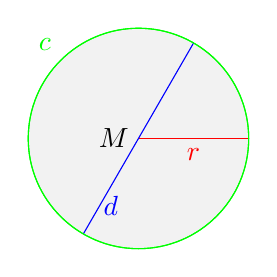
\begin{tikzpicture}
    \newcommand{\R}{1.4}
    \path (240:\R) coordinate (A);
    \path ( 60:\R) coordinate (B);
    \path ( 0:\R) coordinate (C);
    \draw[green,fill=gray!10] (0,0) circle (\R);

    \draw[red] (0,0) -- (C);
    \path[red] ( 0:\R/2) node [below]{$r$};
    \draw[blue] (A) -- (B);
    \path[blue] (240:\R/2) node [below]{$d$};
    \draw[green] (0,0) circle (\R);
    \path[green] (135:\R*1.2) node {$c$};
    \draw[black] (0,0) node [left] {$M$};
\end{tikzpicture}
\end{document}
